%%%%%%%%%%%%%%%%%%%%%%%%%%%%%%%%%%%%%%%%%%%%%%%%%%%%%%%%%%%%%%%%%%%%%%%%%%%%%%%
%                                                                             %
% 03 - Estimación de Precios                                                  %
%                                                                             %
%%%%%%%%%%%%%%%%%%%%%%%%%%%%%%%%%%%%%%%%%%%%%%%%%%%%%%%%%%%%%%%%%%%%%%%%%%%%%%%
\chapter{\textcolor{azulescom}{Estimación de Precios}}

\section{Formulario}
Al acceder a \textit{SkyPrice} lo primero que se presenta es el formulario de
estimación de precios. Este formulario tiene como objetivo recabar la información
necesaria para que los modelos de \textit{Machine Learning} puedan hacer una
predicción de precio de venta de un departamento en la Ciudad de México.

\subsection{Descripción de los campos}
Para poder hacer una predicción de precio de venta de un departamento en la Ciudad
de México, se requiere la siguiente información:

% Lista numerada de campos: Dirección, Tam terreno, Tam construccion, # habitaciones, # baños, # estacionamientos, antigüedad y alcaldía.
\begin{enumerate}
    \item \textbf{Dirección:} La dirección del departamento en la Ciudad de México.
    \item \textbf{Tamaño del terreno:} El tamaño del terreno en metros cuadrados.
    \item \textbf{Tamaño de construcción:} El tamaño de construcción en metros cuadrados.
    \item \textbf{Número de habitaciones:} El número de habitaciones del departamento.
    \item \textbf{Número de baños:} El número de baños del departamento.
    \item \textbf{Número de estacionamientos:} El número de estacionamientos del departamento.
    \item \textbf{Antigüedad:} La antigüedad del departamento en años.
    \item \textbf{Alcaldía:} La alcaldía en la que se encuentra el departamento.
\end{enumerate}

En la figura \ref{fig:formulario} se muestra el formulario de estimación de precios
con números de referencia para cada campo.

\begin{figure}[H]
    \centering
    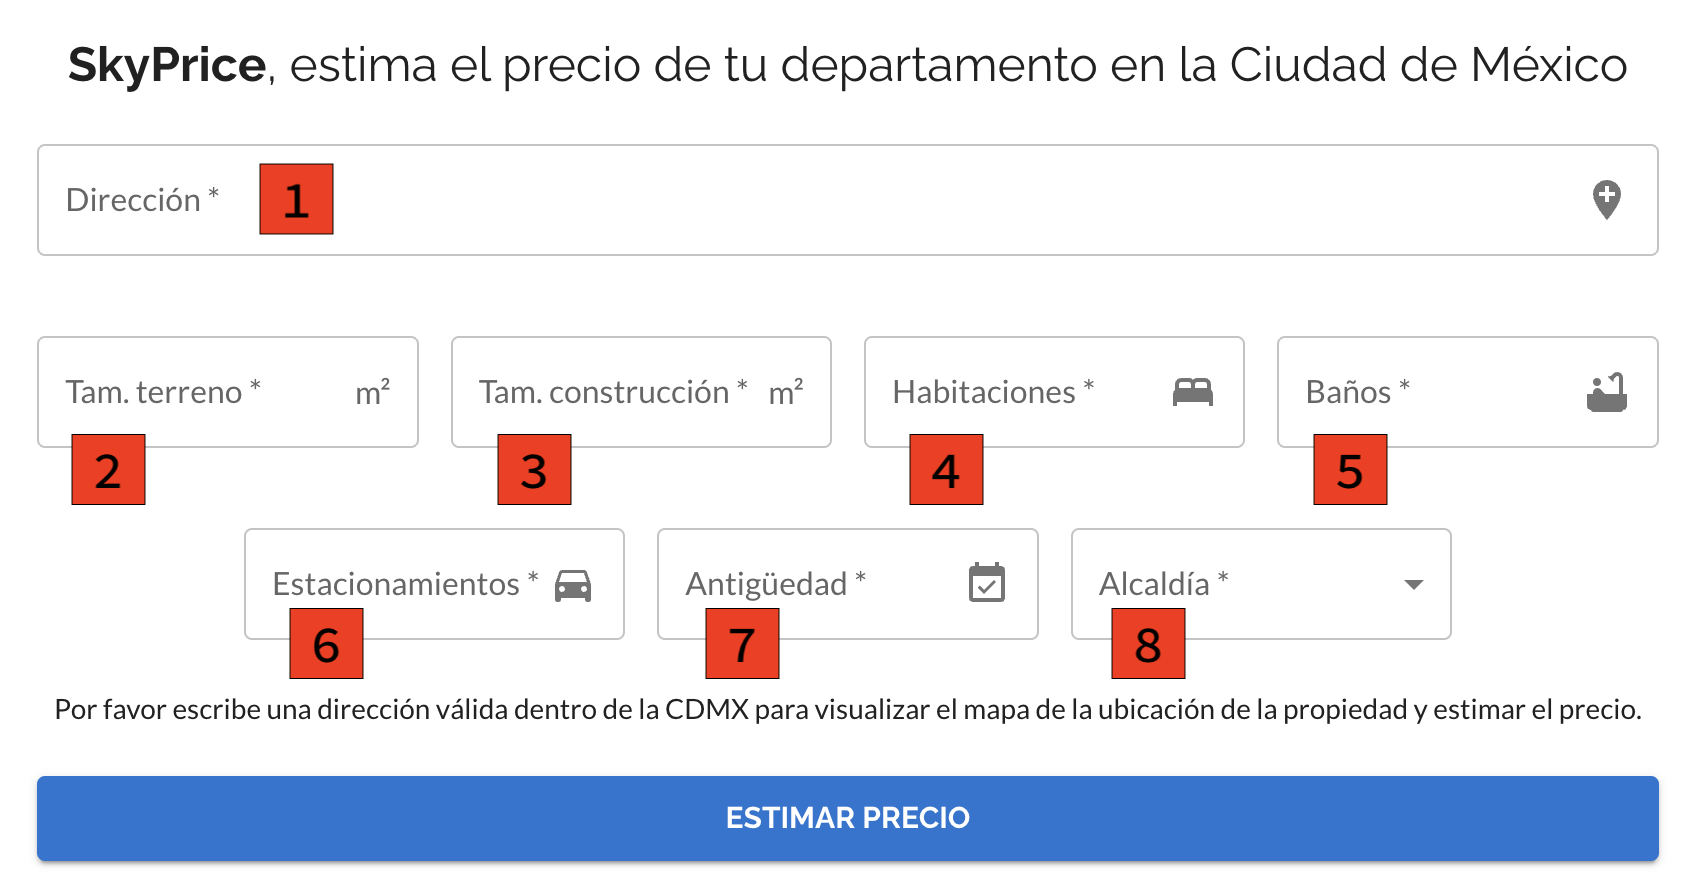
\includegraphics[width=0.8\textwidth]{imagenes/03-estimacion-precios/campos-formulario.png}
    \caption{Campos del formulario de estimación de precios.}
    \label{fig:formulario}
\end{figure}

\subsection{Rangos válidos de entrada}
Para cada campo del formulario de estimación de precios, se tienen los siguientes
rangos válidos de entrada:

\begin{itemize}
    \item \textbf{Dirección:} Cualquier dirección en la Ciudad de México, para esto
    se limitan las coordenadas geográficas dónde el sistema de búsqueda de direcciones
    puede encontrar información.
    \item \textbf{Tamaño del terreno:} 10m\textsuperscript{2} a 1000m\textsuperscript{2}.
    \item \textbf{Tamaño de construcción:} 10m\textsuperscript{2} a 1000m\textsuperscript{2}.
    \item \textbf{Número de habitaciones:} 1 a 10.
    \item \textbf{Número de baños:} 1 a 10, se pueden especificar medos baños.
    \item \textbf{Número de estacionamientos:} 1 a 10.
    \item \textbf{Antigüedad:} 0 a 100 años.
    \item \textbf{Alcaldía:} Cualquiera de las 16 alcaldías de la Ciudad de México.
\end{itemize}

\subsection{Correspondencia de alcaldía y dirección}
Existen situaciones dónde la alcaldía detectada por el sistema de búsqueda de
direcciones (número 1 en la figura \ref{fig:formulario}) no corresponde a la alcaldía en la que se encuentra el departamento.
En estos casos, el usuario puede seleccionar la alcaldía correcta de una lista
desplegable que se muestra en el campo de alcaldía (número 8 en la figura \ref{fig:formulario}).

\section{Resultados}
Una vez que el usuario ha ingresado la información solicitada en el formulario
de estimación de precios, se muestra una página con los resultados de la predicción
de precio de venta del departamento en la Ciudad de México. En la figura \ref{fig:resultados}
se muestra un ejemplo de los resultados de la predicción de precio de venta.

\begin{figure}[H]
    \centering
    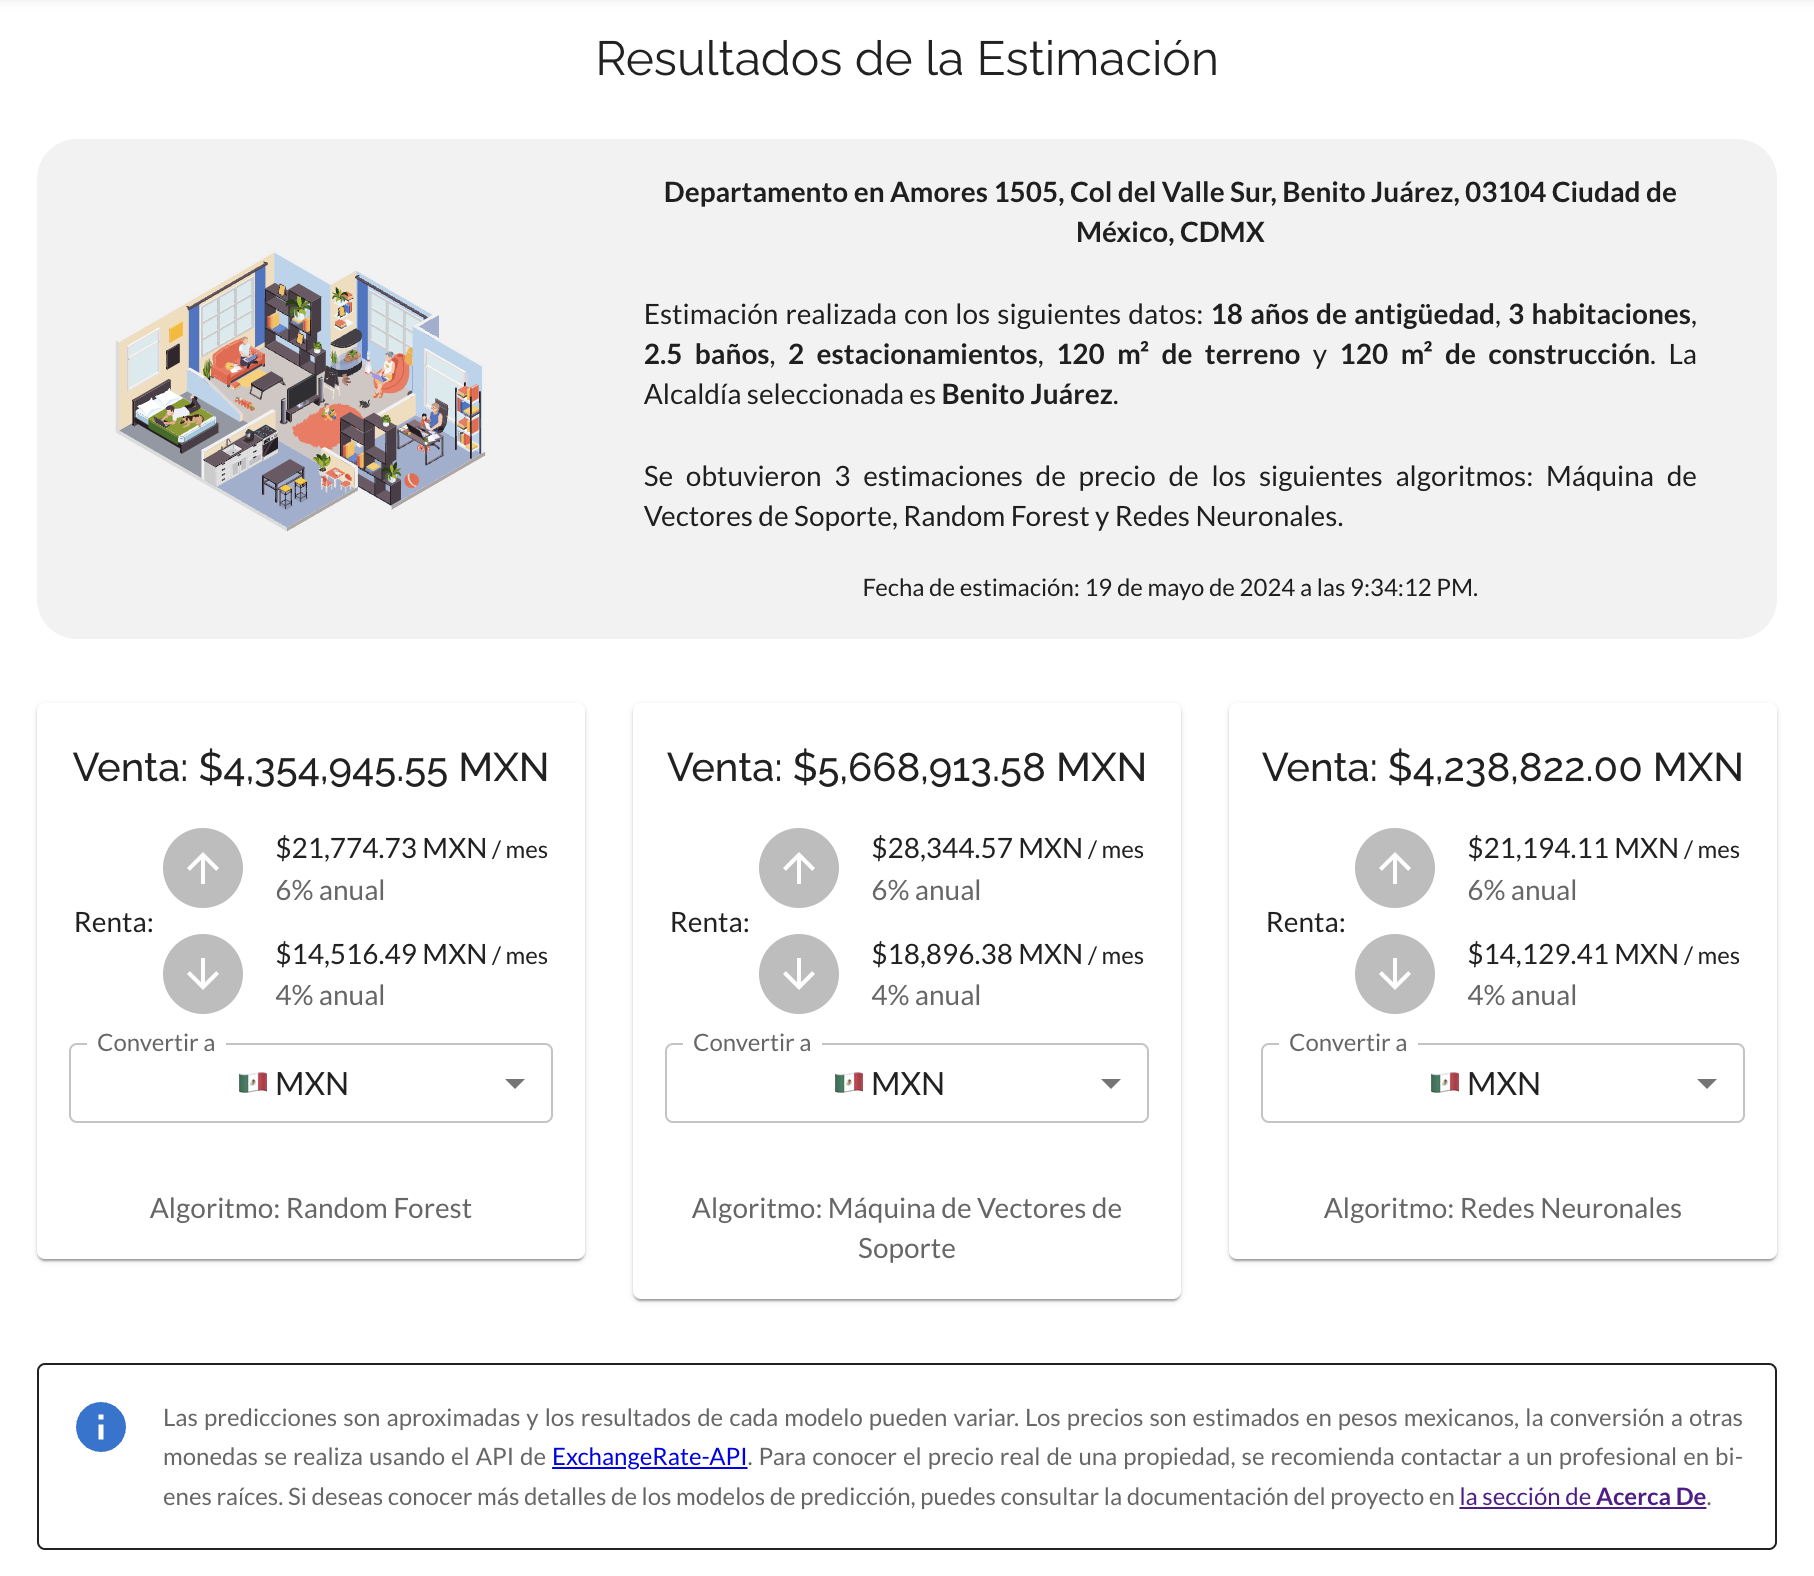
\includegraphics[width=0.8\textwidth]{imagenes/03-estimacion-precios/resultados.png}
    \caption{Resultados de la predicción de precio de venta.}
    \label{fig:resultados}
\end{figure}

\subsection{Texto introductorio}
En la parte superior de la página de resultados se muestra un texto introductorio
que describe el departamento ingresado por el usuario. Este texto incluye la dirección,
tamaño del terreno, tamaño de construcción, número de habitaciones, número de baños,
número de estacionamientos, antigüedad y alcaldía del departamento.

Además, se incluye una nota al pie con la fecha de la predicción realizada. Esto
es importante puesto que si el usuario quisiera compartir la información con alguien
más, es necesario que sepa cuándo se realizó la predicción para entender la validez
de la misma.

\subsection{Predicciones de precios}
En la parte inferior de la página de resultados se muestran las predicciones de
precio de venta del departamento en la Ciudad de México. Estas predicciones se
muestran en tarjetas para cada modelo de \textit{Machine Learning} utilizado en
la predicción.

Cada tarjeta de predicción incluye el nombre del modelo, el precio de venta estimado
del departamento, el precio de renta anualizado al 4\% - 6\% del precio de venta
estimado y una lista de monedas para realizar la conversión de precios a otras
monedas.

\subsection{Aclaración final}
En la parte inferior de la página de resultados se incluye una aclaración final
que indica que los precios de venta y renta son estimados y que pueden variar
dependiendo de las condiciones del mercado inmobiliario en la Ciudad de México.
Además se incluye un enlace a la página de \textit{Acerca de} para que el usuario
pueda obtener más información sobre el sistema de estimación de precios.

